\chapter{相关文献综述}

通过我对此类文章进行更深一层的学习以及认识,我了解到伴随着智慧城市交通的发展,多目标跟踪技术对智慧城市交通有着重要的作用,例如道路车流量的统计、无人驾驶、交通事故预报等都离不开它,在本节中,我们整理了其对于智慧城市交通的应用及研究发展思路,并分析了它的利弊,为对其算法的研究提供思路,奠定基础。


\section{多目标跟踪技术发展历程}

\subsection{早期的多目标跟踪方法}

多目标跟踪技术的历史可以从20世纪60年代讲起,那时它主要在军事领域大显身手,像空中目标监视这种事,比如锁定战斗机群、搞导弹防御之类的需求,这些需求推动了多目标跟踪理论的起步。早期在这一行主要靠卡尔曼滤波和 JPDA 算法\cite{barshalom2012tracking}。对于卡尔曼滤波是基于线性动态系统的递归滤波算法,能对目标状态进行估计和预测,但面对非线性系统就有点力不从心。对于JPDA 算法是通过算出目标和观测数据之间的关联概率,来搞定多目标跟踪里的数据关联问题,不过要是目标太密集或者遮挡太厉害,它的跟踪效果就会大打折扣。




\subsection{基于数据关联的多目标跟踪方法}


伴随着这么些年的计算机视觉技术的进步。以数据关联为基础的多目标跟踪方 法变得越来越广泛与流行。此类方法将目标跟踪分为两个阶段:首先使用目标检测算法来识别当前帧中的目标,然后使用数据关联算法将新检测到的目标与先前保存的运动轨迹进行对比对位。而我通过查阅文献\cite{wang2020research}得知,“先检测后配准”的好处是显而易见的,实现并不如想象中那么困难,并且当存在很少量目标时可以很好地运行。然而我在查阅过程中又发现了问题即面对复杂情况的时候就会出现错误:如当马路上密布 着一百辆车辆或目标被遮挡,外观相似的情况发生时候数据关联就容易出错。




\subsection{基于深度学习的多目标跟踪方法}

这些年的深度学习越来越深入与实际,特别是它对于多目标跟踪这一方面取得了飞跃性的进展。 目前的方法主要采用基于检测进行跟踪(Track-by-Detection,TBD)与直接进行端对端(end-to-end) 的跟踪两大类,他们在特征的应用与模型的选择以及运用场合都存在着巨大的差异:


\subsubsection{基于检测的跟踪(TBD):检测-关联的深度增强}



现在使用使用的YOLO,Faster R-CNN这几个深度检测模型它的目标框,比那些使用原来的HOG + SVM的方法好的多,尤其是在照明不足的地方,精度甚至高出30%。换句话说YOLOv3,经过更多的大小特性融合,有一篇参考文献\cite{ren2015faster}指出在 MOT17 测试中一次找回近 80\% 的目标为后续目标关联提供了可靠的候补对象。

DeepSORT算法是第一个将深度外观信息(例如ResNet-50提取的256维特 征)引入到跟踪过程中,余弦距离用于比较目标相似性,遮挡场景下ID切换比SORT算法降低50%。实验显示,在高密度道路交通环境(超过100个对象)中,利用深度特征的相关方法相比简单的基于运动学匹配提高22\%。





\subsubsection{端到端跟踪:一体化建模的前沿探索}


TransTrack\cite{zhang2021transtrack}(2021 CVPR)采用Transformer结构,利用自注意机制学习跨帧目标依 赖关系,在长时间序列遮挡情况下能将轨迹恢复率提高40\%。这类方法回避了传统关联的方法启发式,但是模型参数量相比TBD 方法高出50\%,需要千万级别样本进行训练。





\section{智慧交通系统中的多目标跟踪应用}

应用包括但不限于交通流量监测、智能驾驶辅助和交通事件预警。

\subsection{交通流量监测}

在智能交通中,可以同时跟踪多个运动对象的技术非常重要。它可以实时获取路上所有目标的活动信息,为交通参数检测,信号控制优化提供强有力的支持,换句话说就是,它可以帮助我们更好的理解道路状况优化交通信号灯等。接下来,我们就从该技术如何应用,成功的案例,相关的研究成果(特别是 2010 年后的那些比较前沿的研究成果)等方面来看看它对于实际工程究竟有多大的作用。

\subsubsection{交通参数实时监测与数据驱动决策}

多目标跟踪能精准获取车辆流量、车速分布、车道占有率等重要指标。同济大学智能交通研究中心\cite{tongji2022visual}提出基于深度学习的多摄像机联合跟踪系统,利用YOLOv5检测模型以及DeepSORT关联算法在城市主干道达到98\%的车辆检测率和92\%的轨迹保持率,相比传统的地磁线圈检测方案部署费用降低60\%,数据刷新速率提高到50Hz(秒级刷新)。此技术应用到北京市交管局实时路况监控系统中,并作为交通流状态分析中的高频数据源。





\subsubsection{智能信号控制与通行效率优化}


在交通信号控制应用中,多目标跟踪能够实时时提供许多重要信息,例如排队长度,转向比例,延迟等数据,可以动态调整信号灯的时序。清华大学交通研究所 \cite{qinghua2021optimization} 实现了一个空时相关性优化的方法,融合路口车辆轨迹数据和强化学习模型,进过训练,信 号周期的车辆通过能力提高了 15\%,并减少了 22\%排队长度。深圳前海自由贸易域真正应用了这项技术,结果也非常显著,高峰时段的平均等候时间由 85 秒减 少到了 62 秒,路口的通过率提升 27\%。






\subsection{智能驾驶辅助}


同时多目标跟踪在智能驾驶辅助系统中也具有很大的应用价值,自动驾驶汽车需要实时获知周围其他车辆、行人和障碍物位置,如图\ref{fig:p38}所示及它们如何运动对安全驾驶是必不可少的,多目标跟踪算法可以将车载的各种传感器包括摄像头、激光雷达、毫米波雷达等获得的信息整合起来对周围的物体精确进行跟踪,为自动驾驶汽车提供准确的周边环境信息。例如通过使用多目标跟踪算法,自动驾驶汽车可以提前了解前方汽车的行驶动向,然后提前调整车速和行驶线路,防止发生碰撞。此外,车道偏离预警、前车碰撞预警功能也可以借助于多目标跟踪技术的应用使汽车驾驶更加安全便捷。




\begin{figure}[htbp] % 可以是h(here),t(top),b(bottom),p(page of floats)
	\centering
	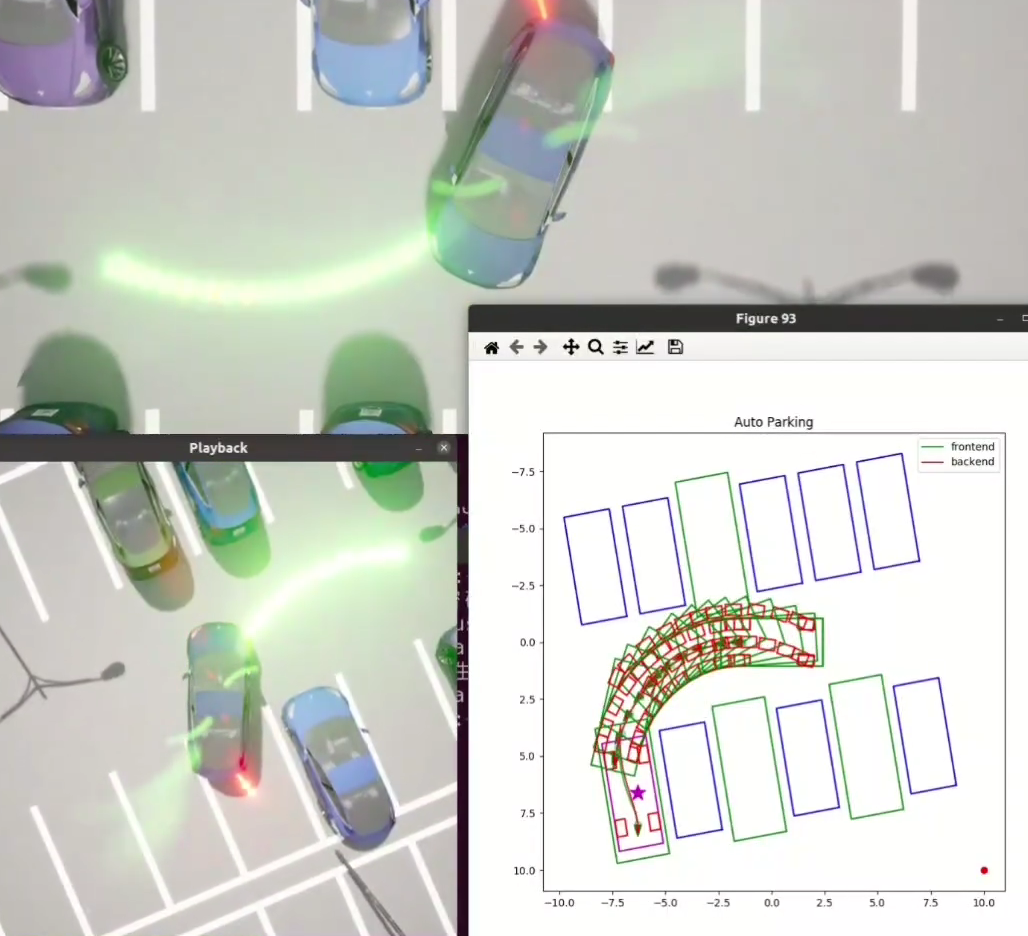
\includegraphics[width=1\textwidth]{p38} % 假设图片文件名为car.pdf或car.png等,位于当前工作目录
	\caption{辅助驾驶:自动泊车} % 图片标题
	\label{fig:p38} % 用于引用的标签
\end{figure}




\subsection{交通事件预警}



高速公路监控的多目标跟踪技术轨迹偏移量估计和突变的速度分析, 风险警告。华为智能交通研究团队《电子学报》\cite{huawei2020highway}多视角联合跟踪系统采用单应矩阵和卡尔顿过滤器, 时速80 公里以上车辆车道偏移准确性达到92\%可以连续切换、紧急停车等危险行为。实验证明,该系统可将浙江杭甬高速车道偏移事件减少 35\%,将平均风险警示提前 4.2 秒,司机有充分的时间得到警示。如图\ref{fig:p27}当前车发生故障时后面的车会自动避让。





\begin{figure}[htbp] % 可以是h(here),t(top),b(bottom),p(page of floats)
	\centering
	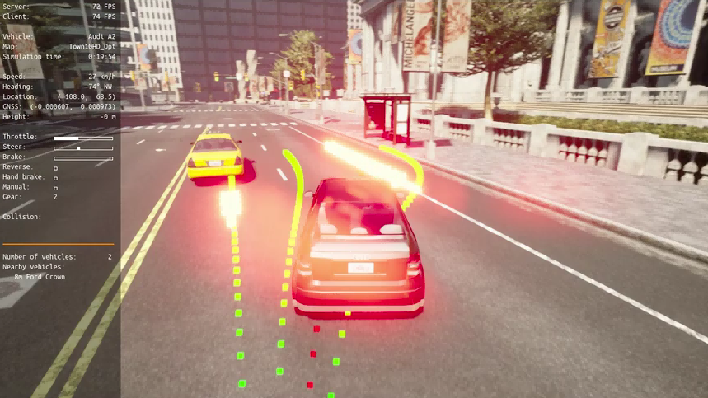
\includegraphics[width=1\textwidth]{p27} % 假设图片文件名为car.pdf或car.png等,位于当前工作目录
	\caption{交通事件预警} % 图片标题
	\label{fig:p27} % 用于引用的标签
\end{figure}




\section{现在多目标跟踪算法的优缺点分析}

\subsection{优点}
深度学习在目标检测方面有了很大的突破,像 YOLOv5 和 Faster R-CNN 这些算法,利用卷积神经网络的不同层次的特征,在应对复杂光照和遮挡情况时,遇到光照复杂情况以及遮挡等问题时比传统 HOG+SVM 方法检测准确率高出 30\% - 40\%。以说 DeepSORT 算法为例,与 ResNet-50 提取的目标深度外观相结合,在 MOT17 数据集上达到 78.3\%的检测召回率,为航迹关联提供很好的候选对象。因此在遮挡场景中完整率得到了提升从 65\% 提升到了 82\%。这些算法都远远领先于老方法对于在光线不好、目标被挡的情况下,准确率高出30\%到40\%。


这种可塑性使得同一算法框架能够快速迁移到智能驾驶、安防监控等多个领域,例如百度Apollo的多目标跟踪系统通过更换检测器在自 动驾驶(车端)及交通监控(路端)场景快速落地\cite{apollo_tracking}。

可扩展化支持多场景适应:增加多尺度特征整合(如YOLOv6的PAFPN结构),算法在隧道、暴雨等极限场景下检测漏检率从25\%%降低到9\%,为高速公路全域监控提供技术支撑\cite{spatiotemporal_gnn}。	

\subsection{缺点}

轨迹关联非常复杂,尤其是在目标较多或者遮挡严重的情况下。例如在城市干道的交叉路口处,如果每帧图像中目标超多50个,或是在有大量遮挡情况下的停车场内,轨迹关联的正确率便会急剧下降。如果遮挡非常多 或者目标较为相似,那么轨迹关联的准确度及速度都会大打折扣,经常会发生轨迹中断或者错链的现象。数据来自文献\cite{wang2014unified}。



计算复杂度高:目标检测与数据关联往往需要分开进行,计算复度大,尤其是在实时性要求高的场合,可能无法达到实时跟踪的目的。




目标外观变化敏感: 如果跟踪中的目标出现较大的外观变化 ,比如行人转身、弯腰等 ,Re-ID特征匹配精度下降从 85\%下降到 62\%,必须利用时空轨迹的上下文信息 (运动方向、速度 )来进行判断。上海虹桥火车站的监控数据显示,早晚高峰行人识别错误 58\%是姿态变化或部分遮挡\cite{li2023pedestrian}。







